%% FullCourse_10Lecs -- Lecture 2, Topic 2.1: ML and the Predictive Stack
%% New deck (Lec02_What_is_AI_New): predictive-stack half of the "What is AI" split.
%% OVERVIEW altitude: intuitive (how it works + what it is used for, esp. in
%% economics), not a technical ML course (mechanics are taught in Lec 3-9).
%% Reuses the evolution/landscape frames, repositions RL as a closing bridge to
%% Arc 1, and adds an AI Snake Oil (Narayanan & Kapoor, 2024) caution section on
%% why PREDICTIVE AI fails (COMPAS; Fragile Families; Table 2.1).

%% Shared preamble for the FullCourse_10Lecs topic decks.
%%
%% Each topic .tex \input's this file, then defines its own \title, \date
%% override (if any), \graphicspath, and \begin{document}.
%%
%% Reconstructed verbatim from the inlined copy preserved in
%% Lec10_Case_Studies/Lec10_T8_Case6_DeepRamsey.tex (lines 23-190), which is
%% explicitly annotated there as "from ../shared_preamble.tex, copied verbatim".
%% Base preamble matches MiniCourse_8hr/Slides/shared_preamble.tex; this version
%% additionally provides \sectiondivider, the conceptbox/cautionbox/examplebox/
%% takeawaybox tcolorboxes, and \compacttables used across the split decks.

\documentclass[10pt,english,aspectratio=169]{beamer}

\usepackage{ae,aecompl}
\usepackage[T1]{fontenc}
\usepackage{textcomp}
\usepackage[utf8]{inputenc}
\usepackage{babel}
\usepackage{datetime2}

\setcounter{secnumdepth}{3}
\setcounter{tocdepth}{3}

\usepackage{amsmath, amssymb, amsthm, graphicx}
\usepackage{booktabs, multirow}
\usepackage{tikz}
\usepackage{pgfplots}
\pgfplotsset{compat=1.16}
\usepackage[most]{tcolorbox}
\tcbuselibrary{skins, breakable, theorems}
\usepackage{listings}
\usepackage{xcolor}

\lstset{
  basicstyle=\ttfamily\small,
  keywordstyle=\color{blue!80!black}\bfseries,
  commentstyle=\color{green!50!black}\itshape,
  stringstyle=\color{orange!80!black},
  backgroundcolor=\color{gray!8},
  frame=single,
  rulecolor=\color{gray!40},
  breaklines=true,
  showstringspaces=false,
  numbers=none,
}

\lstdefinestyle{pythonstyle}{
    language=Python,
    basicstyle=\ttfamily\footnotesize,
    keywordstyle=\color{blue!80!black}\bfseries,
    commentstyle=\color{green!50!black}\itshape,
    stringstyle=\color{orange!80!black},
    frame=single,
    breaklines=true,
    showstringspaces=false,
    numbers=left,
    numbersep=5pt,
    numberstyle=\tiny\color{gray},
    backgroundcolor=\color{gray!8},
    rulecolor=\color{gray!40}
}

\ifx\hypersetup\undefined
  \AtBeginDocument{%
    \hypersetup{bookmarks=false,breaklinks=true,pdfborder={0 0 0},colorlinks=true,
      linkcolor=DarkText,urlcolor=RedTitle}%
  }
\else
  \hypersetup{bookmarks=false,breaklinks=true,pdfborder={0 0 0},colorlinks=true,
    linkcolor=DarkText,urlcolor=RedTitle}%
\fi

\makeatletter
\newcommand\makebeamertitle{%
  \begin{frame}[plain]
    \vspace*{1.0cm}
    \centering
    {\usebeamerfont{title}\usebeamercolor[fg]{title}\inserttitle\par}
    \vspace{1.0cm}
    {\usebeamerfont{author}\usebeamercolor[fg]{author}\insertauthor\par}
    \vspace{0.2cm}
    {\usebeamerfont{date}\usebeamercolor[fg]{date}\insertdate\par}
  \end{frame}}%
\AtBeginDocument{%
  \let\origtableofcontents=\tableofcontents
  \def\tableofcontents{\@ifnextchar[{\origtableofcontents}{\gobbletableofcontents}}
  \def\gobbletableofcontents#1{\origtableofcontents}%
}

\usetheme{metropolis}
\usefonttheme{professionalfonts}

\definecolor{LightGray}{RGB}{230,230,230}
\definecolor{RedTitle}{RGB}{0,0,200}
\definecolor{VeryLightGray}{RGB}{245,245,245}
\definecolor{DarkText}{RGB}{0,0,0}

\setbeamercolor{background canvas}{bg=white}
\setbeamercolor{title}{fg=RedTitle}
\setbeamercolor{author}{fg=DarkText}
\setbeamercolor{date}{fg=DarkText}
\setbeamercolor{frametitle}{bg=VeryLightGray,fg=DarkText}
\setbeamercolor{normal text}{fg=DarkText}
\setbeamerfont{title}{size=\large}

\setbeamersize{text margin left=5mm, text margin right=5mm}
\addtobeamertemplate{frametitle}{}{\vspace{-0.5em}}
\newcommand{\reducevspace}{\vspace{-0.5cm}}

% Shared section divider and box styles for split topic decks.
\newcommand{\sectiondivider}[2]{%
\begin{frame}[plain,noframenumbering]
\begin{center}
\vfill
{\Large\textbf{#1}\par}
\vspace{0.35cm}
{\normalsize #2\par}
\vfill
\end{center}
\end{frame}
}

\newtcolorbox{conceptbox}[1][]{
  colback=blue!3,
  colframe=RedTitle!55,
  boxrule=0.35mm,
  arc=1mm,
  left=2mm,
  right=2mm,
  top=1mm,
  bottom=1mm,
  #1
}
\newtcolorbox{cautionbox}[1][]{
  colback=red!3,
  colframe=red!50!black,
  boxrule=0.35mm,
  arc=1mm,
  left=2mm,
  right=2mm,
  top=1mm,
  bottom=1mm,
  #1
}
\newtcolorbox{examplebox}[1][]{
  colback=green!3,
  colframe=green!45!black,
  boxrule=0.35mm,
  arc=1mm,
  left=2mm,
  right=2mm,
  top=1mm,
  bottom=1mm,
  #1
}
\newtcolorbox{takeawaybox}[1][]{
  colback=VeryLightGray,
  colframe=RedTitle!55,
  boxrule=0.35mm,
  arc=1mm,
  left=2mm,
  right=2mm,
  top=1mm,
  bottom=1mm,
  #1
}
\newcommand{\compacttables}{\renewcommand{\arraystretch}{1.15}}

\setbeamertemplate{navigation symbols}{}
\setbeamertemplate{footline}{%
  \hfill%
  \usebeamercolor[fg]{page number in head/foot}%
  \usebeamerfont{page number in head/foot}%
  \insertframenumber\,/\,\inserttotalframenumber\kern1em\vskip2pt%
}

\makeatother

\author{Zhigang Feng}
% "date with time": compile timestamp so each build is identifiable.
\date{\today\ \DTMcurrenttime}


\graphicspath{{./figures/}{./pic/}{../../MiniCourse_8hr/Slides/Module1_ML_Foundations/pic/}{../}}

% Suppress the redundant auto-generated metropolis section page; the
% \sectiondivider frames below are the dividers we keep.
\metroset{sectionpage=none}
\usetikzlibrary{positioning,arrows.meta,shapes,calc}
%% Lec02 shared MAP slide: "one map, two acts" recurring diagram.
%% Input this file AFTER ../shared_preamble.tex (needs RedTitle, VeryLightGray,
%% DarkText) and AFTER \usetikzlibrary{positioning,arrows.meta,shapes,calc}.
%% Call \LecTwoMap{k} inside a frame, where k in {1,2} highlights the current
%% act ("you are here") and k = 0 renders the closing reprise with both acts
%% checked green (used by T2's closing frame).
%% Filename deliberately does NOT match the build glob Lec*_T*.tex, so the build
%% script never tries to compile it standalone.
%%
%% The two acts are the lecture's story: PREDICT -> GENERATE, i.e. the
%% predictive stack (ML pillars + deep learning + where it fails) and the
%% generative/agentic stack (LLMs + agents + where it fails) --- and the two
%% acts point at the course's two arcs (dynamics: Lec03-06; language: Lec07-09).

\newcommand{\LecTwoMap}[1]{%
% Precompute per-box style selectors; TikZ option lists are comma-split before
% TeX conditionals run, so \ifnum must not sit inside a [...] options list.
\ifnum#1=0
  \tikzset{lmapa/.style={lmapdone}, lmapb/.style={lmapdone}}%
\else
  \tikzset{lmapa/.style={}, lmapb/.style={}}%
  \ifnum#1=1 \tikzset{lmapa/.style={lmapcur}}\fi
  \ifnum#1=2 \tikzset{lmapb/.style={lmapcur}}\fi
\fi
\begin{center}
\begin{tikzpicture}[
    act/.style={rectangle, rounded corners, draw=black!60, fill=VeryLightGray,
        minimum width=4.6cm, minimum height=1.0cm, text width=4.45cm,
        align=center, font=\small, text=DarkText},
    lmapcur/.style={draw=RedTitle, very thick, fill=orange!20},
    lmapdone/.style={draw=green!45!black, thick, fill=green!10},
    q/.style={font=\tiny\itshape, text width=4.6cm, align=center, text=black!70},
    barlab/.style={font=\tiny\bfseries, text=black!65},
    sat/.style={rectangle, rounded corners, draw=black!45, dashed, fill=white,
        text width=5.2cm, align=center, font=\tiny, text=black!70,
        minimum height=0.5cm},
    arr/.style={-{Stealth[length=2.4mm]}, thick, gray!60}
]
    % --- two act boxes ---
    \node[act, lmapa] (a1) at (0,0)
        {\textbf{2.1\ \ PREDICT}\\[1pt] \tiny three pillars $\cdot$ deep learning $\cdot$ where it fails};
    \node[act, lmapb] (a2) at (6.8,0)
        {\textbf{2.2\ \ GENERATE}\\[1pt] \tiny LLMs $\cdot$ agents $\cdot$ where it fails};
    \draw[arr] (a1) -- (a2);
    % --- the student question each act answers ---
    \node[q] at (0,-0.98)   {what is AI/ML --- and when\\ does prediction go wrong?};
    \node[q] at (6.8,-0.98) {what changed with LLMs and\\ agents --- and what still fails?};
    % --- "you are here" marker above the current act ---
    \ifnum#1=1 \node[font=\scriptsize\bfseries, text=RedTitle] at (0,1.02)
        {you are here\ $\blacktriangledown$};\fi
    \ifnum#1=2 \node[font=\scriptsize\bfseries, text=RedTitle] at (6.8,1.02)
        {you are here\ $\blacktriangledown$};\fi
    \ifnum#1=0 \node[font=\scriptsize\bfseries, text=green!45!black] at (3.4,1.02)
        {both acts complete};\fi
    % --- bottom band: each act's caution centerpiece (the lecture's spine) ---
    \fill[blue!10]   (-2.4,-1.78) rectangle (2.4,-1.45);
    \fill[orange!16] (4.4,-1.78)  rectangle (9.2,-1.45);
    \node[barlab] at (0,-1.615)   {FIVE REASONS PREDICTIVE AI FAILS};
    \node[barlab] at (6.8,-1.615) {WHAT TASK $\cdot$ WHAT DATA $\cdot$ WHAT CLAIM};
    % --- dashed satellites: the two acts feed the course's two arcs ---
    \node[sat] at (0,-2.45)
        {\textit{upstream:} Lec01 --- AI as cognitive capital, already doing research};
    \node[sat] at (6.8,-2.45)
        {\textit{downstream:} Act 1 $\to$ Arc 1 (Lec03--06, dynamics); Act 2 $\to$ Arc 2 (Lec07--09, language \& agents)};
\end{tikzpicture}
\end{center}
}


\title[AI for Econ Research]{AI for Economic Research: Dynamic Models, Language, and Agents\\
Lecture 2.1: ML and the Predictive Stack}

\begin{document}

\makebeamertitle

%=============================================================================
\begin{frame}{Lecture 2 in One Map}
\textbf{One lecture, two decks, one taxonomy: the predictive stack and the generative stack --- what each is, how it is used in economics, and \emph{where each fails}.}

\LecTwoMap{1}

\vspace{0.05cm}
\footnotesize\textit{\textbf{Act 2.1 (here)} builds the predictive stack: the AI evolution, the three pillars of ML with deep learning as the engine, the caution file (COMPAS, Fragile Families, five reasons --- the Lucas critique in ML clothing), and the RL bridge to Arc 1. An intuitive map only --- the mechanics arrive in Lec.\ 3--9.}
\end{frame}

%=============================================================================
\section{AI Evolution and Landscape}

\sectiondivider{AI Evolution and Landscape}{From rule-based systems to the agentic era}

\begin{frame}{AI Evolution: Foundations to Deep Learning}
\begin{itemize}
    \item \textbf{Foundations (1950s)}:
    \begin{itemize}
        \item Alan Turing introduces the ``universal machine'' and the Turing Test, establishing the theoretical bedrock (Turing, 1950).
        \item John McCarthy coins ``Artificial Intelligence'' at the Dartmouth Conference (McCarthy et al., 1956).
    \end{itemize}

    \medskip
    \item \textbf{The Deep Learning Era (2010s)}:
    \begin{itemize}
        \item Widespread adoption of neural networks and backpropagation enables superhuman performance in specific domains (LeCun, Bengio, \& Hinton, 2015).
        \item ImageNet, AlphaGo, AlphaFold --- AI beats humans at tasks once deemed impossible.
    \end{itemize}
\end{itemize}
\end{frame}

\begin{frame}{AI Evolution: Generative to Agentic AI}
\begin{itemize}
    \item \textbf{The Generative Era (2017--2024)}:
    \begin{itemize}
        \item The Transformer architecture (Vaswani et al., 2017) and Large Language Models (GPT, Claude) shift focus to general-purpose reasoning and generative capabilities.
        \item Multimodal unification: vision, language, and code in a single model (GPT-4o, Claude~3.5/4, Gemini~2).
    \end{itemize}

    \medskip
    \item \textbf{The Reasoning \& Agentic Era (2024--)}:
    \begin{itemize}
        \item \emph{Reasoning models} (OpenAI o1/o3, Claude thinking, DeepSeek-R1) trade inference compute for chains of thought --- partial answer to Chollet's ARC critique (Chollet, 2019; ARC Prize 2024).
        \item \emph{Open-source frontier} (Llama 3+, DeepSeek, Qwen) closes the gap with proprietary; lowers cost of academic experimentation by orders of magnitude.
        \item \emph{Agentic AI}: models act autonomously, plan multi-step tasks, write and execute code, drive research workflows (Lec.\ 9).
    \end{itemize}
\end{itemize}
\end{frame}

\begin{frame}{AI Landscape}
\begin{center}
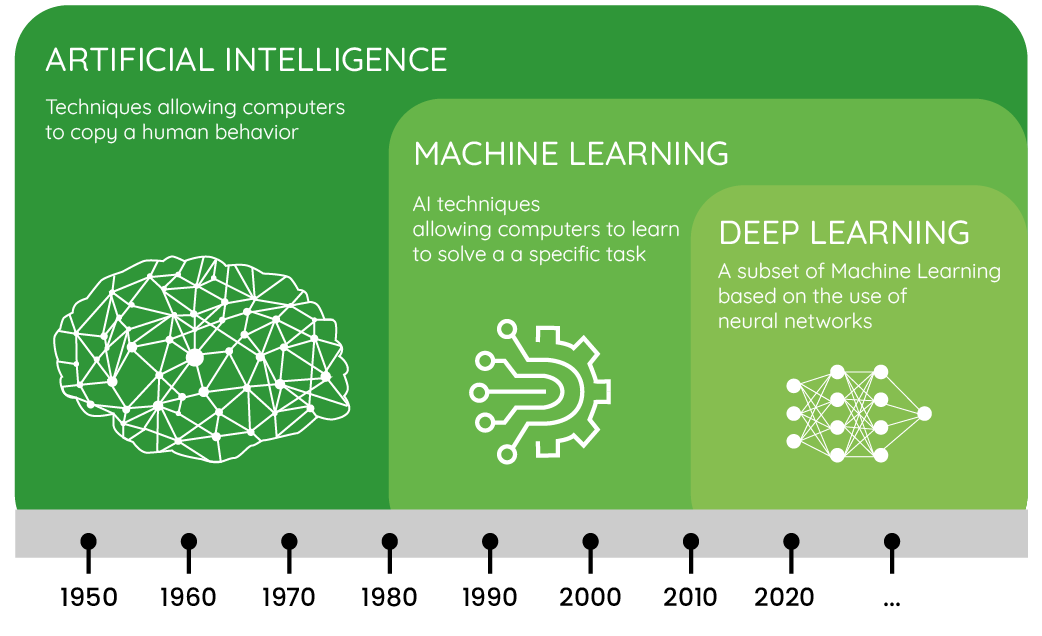
\includegraphics[width=13cm,totalheight=7cm]{figures/AI}
\par\end{center}
\end{frame}

%=============================================================================
\section{Three Pillars of Machine Learning}

\sectiondivider{Three Pillars of Machine Learning}{Supervised, unsupervised, reinforcement --- one engine underneath}

\begin{frame}{Machine Learning}
\begin{center}
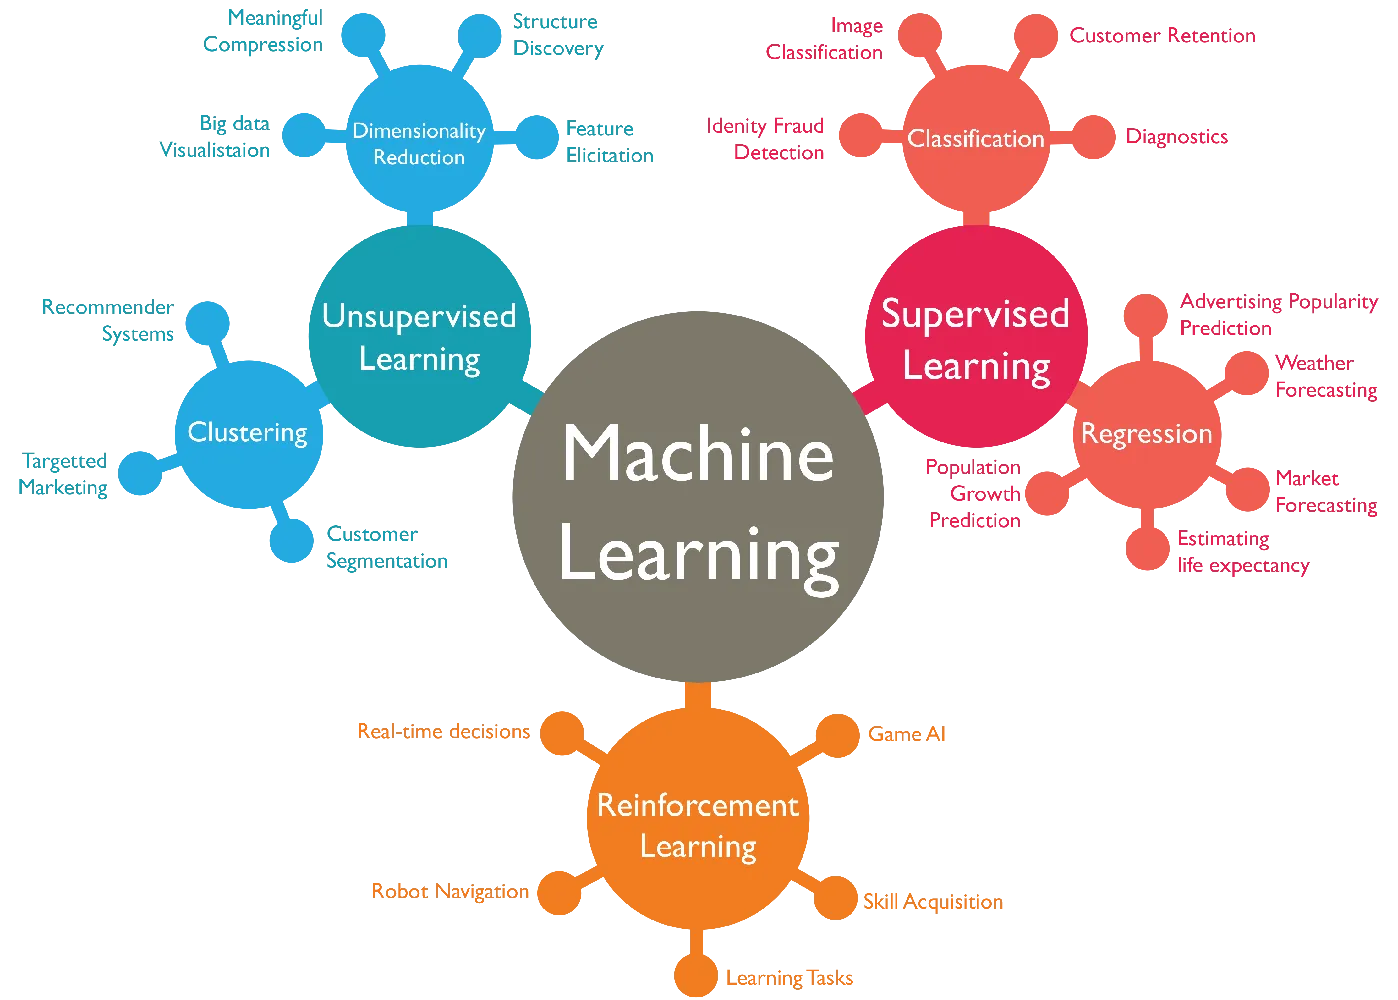
\includegraphics[width=13cm,totalheight=7cm]{figures/machine_learning}
\par\end{center}
\end{frame}

\begin{frame}{The Three Pillars of Machine Learning}
\textbf{Three ways a machine can ``learn'' from data:}
\begin{itemize}
\item \textbf{Supervised learning} --- learn from \emph{labeled examples}.
\begin{itemize}
    \item You provide inputs \emph{and} the right answers; it learns to predict the answer for new inputs.
    \item In economics: predicting recessions, income, credit risk.
\end{itemize}

\medskip
\item \textbf{Unsupervised learning} --- find \emph{patterns without labels}.
\begin{itemize}
    \item No answer key; it organizes the data by its own structure.
    \item In economics: discovering consumer types, themes in earnings calls.
\end{itemize}

\medskip
\item \textbf{Reinforcement learning (RL)} --- learn by \emph{trial and error}.
\begin{itemize}
    \item An agent acts, gets rewards, and improves; the foundation is the Bellman equation.
    \item In economics: optimal policy, dynamic pricing (the dynamic-macro arc, Lec.\ 4--6).
\end{itemize}
\end{itemize}
\vspace{1mm}
{\footnotesize\textit{This deck focuses on the two \emph{predictive} pillars; RL returns as the bridge to Arc 1.}}
\end{frame}

\begin{frame}{Supervised Learning: Learning from Labeled Examples}
\begin{itemize}
\item \textbf{The idea.} Show the model many examples, each an input paired with the \emph{correct answer}. It learns a rule that generalizes to inputs it has never seen.
\medskip
\item \textbf{Two flavors:}
\begin{itemize}
    \item \emph{Regression} --- predict a \textbf{number}: GDP growth, a wage, a house price.
    \item \emph{Classification} --- predict a \textbf{category}: recession or not? loan default or not?
\end{itemize}
\medskip
\item \textbf{How it ``learns.''} It simply tunes itself so its predictions match the known answers as closely as possible --- no hand-coded rules.
\end{itemize}
\vfill
\begin{conceptbox}\footnotesize
\textbf{Intuition:} supervised learning is curve-fitting taken to its limit --- flexible enough to find patterns a human would never write down by hand, as long as you can supply labeled examples.
\end{conceptbox}
\end{frame}

\begin{frame}{Supervised Learning in Economics}
\textbf{Where labeled examples are plentiful, supervised learning is a natural fit:}
\smallskip
\begin{itemize}
    \item \textbf{Nowcasting:} predict GDP or inflation from high-frequency and alternative data (card spending, satellite night-lights).
    \item \textbf{Markets:} predict earnings surprises from SEC filings (text $\to$ returns).
    \item \textbf{Credit:} score loan default or firm failure from credit and balance-sheet history.
    \item \textbf{Labor:} predict individual wages from demographic and job features.
\end{itemize}
\vfill
\begin{takeawaybox}\footnotesize
\textbf{Why economists are well-placed:} rich, \emph{labeled} administrative datasets (tax, credit, employment) are exactly what supervised learning needs. Mechanics and a hands-on lab: \textbf{Lec.\ 3}.
\end{takeawaybox}
\end{frame}

\begin{frame}{Unsupervised Learning: Finding Structure Without Labels}
\begin{itemize}
\item \textbf{The idea.} No answer key. The model groups or organizes the data using only its own structure --- useful when the ``right'' categories are unknown or contested.
\medskip
\item \textbf{Clustering} --- group similar units together.
\begin{itemize}
    \item Sort firms, consumers, or households into \emph{types} ($k$-means, mixtures).
    \item In economics: consumer segments from spending panels; firm clusters from Compustat.
\end{itemize}
\medskip
\item \textbf{Topic modeling} --- discover recurring \emph{themes} in text.
\begin{itemize}
    \item Surface the latent topics in a corpus (LDA).
    \item In economics: FOMC minutes, congressional speeches, earnings calls.
\end{itemize}
\end{itemize}
\end{frame}

\begin{frame}{Unsupervised Learning: Compression and Embeddings}
\begin{itemize}
\item \textbf{Dimensionality reduction} --- summarize many variables with a few.
\begin{itemize}
    \item Intuition (PCA): \emph{find the few ``dials'' that explain most of the variation}.
    \item In economics: extract a handful of macro factors from hundreds of series (FRED-MD).
\end{itemize}
\medskip
\item \textbf{Word embeddings} --- turn words into \emph{vectors that capture meaning}.
\begin{itemize}
    \item Similar meanings land near each other: ``king $-$ man $+$ woman $\approx$ queen.''
    \item In economics: measure ideological shift in political text over time.
\end{itemize}
\end{itemize}
\vfill
\begin{conceptbox}\footnotesize
Word embeddings \emph{are} learned dimensionality reduction for language --- the foundation Lec.\ 7 builds into transformers and LLMs.
\end{conceptbox}
\end{frame}

%=============================================================================
\section{Deep Learning: the Engine}

\sectiondivider{Deep Learning: the Engine}{What a neural network is, how it learns, why now}

\begin{frame}{Deep Learning: What Is a Neural Network?}
\begin{itemize}
\item A neural network stacks many simple units (``neurons'') in \textbf{layers}.
\medskip
\item Each neuron takes a weighted sum of its inputs and passes it through a simple nonlinear ``switch'':
\[
z = \sigma\!\big(\underbrace{w_1 x_1 + \cdots + w_n x_n + b}_{\text{weighted sum of inputs}}\big)
\]
--- that is the \emph{only} formula you need today; everything else is many of these wired together.
\medskip
\item Stacking layers lets the network build ever more abstract features: in vision, \emph{edges $\to$ shapes $\to$ objects}.
\end{itemize}
\vfill
\begin{takeawaybox}\footnotesize
\textbf{Why it matters:} a neural network is an extremely \emph{flexible function approximator} --- with enough data it can represent very complex input$\to$output relationships (universal approximation; Cybenko, 1989). That flexibility is what we exploit to solve hard macro models in Lec.\ 4.
\end{takeawaybox}
\end{frame}

\begin{frame}{How a Neural Network Learns}
\textbf{Learning is one simple loop, repeated millions of times:}
\smallskip
\begin{enumerate}
    \item \textbf{Predict} --- run an example through the network.
    \item \textbf{Measure the error} --- how far is the prediction from the right answer?
    \item \textbf{Nudge the weights} a little in the direction that \emph{reduces} the error.
    \item \textbf{Repeat} on the next batch of examples.
\end{enumerate}
\smallskip
\begin{itemize}
\item Step 3 is \emph{gradient descent} --- intuitively, ``roll downhill'' on the error surface.
\item Modern software (PyTorch) computes all the derivatives \emph{automatically}, so you never do the calculus by hand.
\end{itemize}
\vfill
\begin{conceptbox}\footnotesize
\textbf{Economic analogy:} like a firm adjusting its input mix to minimize cost, the network adjusts its weights to minimize prediction error. (Backpropagation, optimizers, and regularization: \textbf{Lec.\ 3}.)
\end{conceptbox}
\end{frame}

\begin{frame}{Why Now: Data, Compute, and Algorithms}
\textbf{Deep learning is decades old --- three ingredients made it work only recently (LeCun's ``three conditions''):}
\smallskip
\begin{enumerate}
    \item \textbf{Data} --- internet-scale datasets (ImageNet's 14M images; trillions of words of text).
    \medskip
    \item \textbf{Compute} --- cheap, massively parallel hardware (GPUs; later TPUs).
    \medskip
    \item \textbf{Algorithms} --- better training tricks (ReLU activations, dropout, the Adam optimizer).
\end{enumerate}
\vfill
\begin{takeawaybox}\footnotesize
None of the three alone was enough. Their \emph{coincidence} in the 2010s is what turned neural networks from a curiosity into the dominant technology.
\end{takeawaybox}
\end{frame}

\begin{frame}{Scaling and the ``Tokenization of Everything''}
\begin{itemize}
\item \textbf{Scaling laws (Kaplan et al., 2020).} Bigger model $+$ more data $+$ more compute $\to$ \emph{predictably} better performance --- within limits. ``Bigger is better,'' for now.
\medskip
\item \textbf{Tokenization of everything.} Text, images, audio, code --- even protein sequences --- are all turned into \emph{tokens} and processed by one architecture, the \textbf{Transformer}.
\medskip
\item A single design now powers most state-of-the-art AI; the demand for compute is why \emph{``GPUs are the new oil''} (and why Nvidia's revenue tracks the AI boom).
\end{itemize}
\end{frame}

%=============================================================================
\section{Caution: Why Predictive AI Fails}

\sectiondivider{Caution: Why Predictive AI Fails}{COMPAS, Fragile Families, and five reasons --- the Lucas critique in ML clothing}

\begin{frame}{Two Kinds of AI, Two Kinds of Failure}
\textbf{A distinction we carry through both decks --- and the central thesis of \emph{AI Snake Oil}:}
\begin{itemize}
    \item \textbf{Predictive AI} forecasts an \emph{outcome} --- \emph{Will this defendant reoffend? Will this loan default?} This is the supervised/unsupervised stack of \emph{this} deck.
    \medskip
    \item \textbf{Generative AI} produces \emph{content} --- text, images, code. That is the subject of \textbf{T2.2}.
\end{itemize}
\medskip
\begin{cautionbox}\footnotesize
Both are powerful, but they fail \emph{for different reasons}. Predictive AI tends to fail because the future simply is not in the data; generative AI fails by producing fluent-but-false or harmful content (T2.2). We start with a deployed \emph{predictive} system.
\end{cautionbox}
\vspace{1mm}
{\scriptsize\textit{Source for this caution section: Arvind Narayanan \& Sayash Kapoor, \textbf{AI Snake Oil: What Artificial Intelligence Can Do, What It Can't, and How to Tell the Difference} (Princeton Univ.\ Press, 2024). Their thesis --- there is almost nothing true of \emph{all} AI at once; do not paint it with a single brush.}}
\end{frame}

\begin{frame}{COMPAS: When Predictive AI Meets the Real World}
\textbf{COMPAS} --- a 137-question pretrial tool predicting failure-to-appear / re-arrest within two years, used in U.S.\ courts:
\smallskip
\begin{itemize}\footnotesize
    \item ProPublica's 2016 Broward County study ($\sim$10{,}000 people): \textbf{relative accuracy only 64\%} --- and 50\% is a random coin flip.
    \item \textbf{45\% of Black defendants who did \emph{not} reoffend} were flagged high-risk, vs.\ \textbf{23\% of White} --- misclassified at twice the rate.
    \item A 2-feature model (age $+$ prior offenses) was about \emph{as accurate} as all 137 questions.
\end{itemize}
\begin{cautionbox}
\footnotesize
\textbf{Label bias --- the claimed target $\neq$ the measured target.} COMPAS says it predicts \emph{crime}, but its data only record \emph{arrests}; policing is racially skewed, so the model learns the biases of policing, not criminality. (Narayanan \& Kapoor, 2024)
\end{cautionbox}
\end{frame}

\begin{frame}{Predicting Human Futures: The Fragile Families Challenge}
\textbf{The best-case test of social prediction --- and it still failed.}
\smallskip
\begin{itemize}
    \item \textbf{The design (Salganik \& McLanahan, Princeton).} A scientific mass collaboration: \textbf{$\sim$4{,}000 children} followed from birth, \textbf{$\sim$10{,}000 features each}, \textbf{160 teams}, the most advanced AI available.
    \medskip
    \item \textbf{The task.} Predict age-15 outcomes --- GPA, eviction, material hardship --- on a \textbf{held-out test set} the teams never saw (so \emph{no data leakage}, unlike most prediction studies).
    \medskip
    \item \textbf{The result.} The best models were \emph{barely better than a coin flip} --- and \emph{no better than a simple 4-feature baseline regression}.
\end{itemize}
\vfill
\begin{cautionbox}\footnotesize
Tens of thousands of data points, 160 teams, the most advanced AI --- and none could out-predict a decades-old regression with four variables. \emph{Why?} $\rightarrow$ next slide. (Narayanan \& Kapoor, 2024; Salganik et al., \emph{PNAS} 2020)
\end{cautionbox}
\end{frame}

\begin{frame}{Why Predicting Human Futures Fails --- Even in the Best Case}
\begin{itemize}
    \item \textbf{Irreducible chance.} Lives turn on events no survey records --- one child improved because ``a supportive neighbor counseled them and fed them blueberries.'' Such shocks are, by definition, unlearnable from data.
    \medskip
    \item \textbf{Non-stationarity.} Social data are noisy and shift over time --- yesterday's pattern need not hold tomorrow (the same regime-change problem as the predictive failures above).
\end{itemize}
\medskip
\begin{conceptbox}\footnotesize
\textbf{Salganik's ``eight-billion problem.''} To predict a life, a model must have \emph{already seen enough sufficiently-similar lives} to learn the pattern. But the number of distinct, relevant life-trajectories --- every combination of family, place, timing, and luck --- is astronomically larger than the $\sim$8 billion people alive. Most lives are effectively \emph{unique}: there is no close ``neighbor'' in the data to learn from. \emph{More data cannot fix this} --- there may simply not be enough people on Earth.
\end{conceptbox}
\smallskip
{\footnotesize\textit{The binding limit is not the algorithm --- it is the intrinsic predictability of human lives. (Narayanan \& Kapoor, 2024, ch.\ 3)}}
\end{frame}

\begin{frame}{Five Reasons Predictive AI Fails}
\compacttables
\begin{center}\footnotesize
\renewcommand{\arraystretch}{1.1}
\begin{tabular}{p{6.2cm}p{6.0cm}}
\toprule
\textbf{Reason} & \textbf{Example} \textit{(AI Snake Oil, Tbl.\ 2.1)} \\
\midrule
1. A good \emph{prediction} can still produce a \emph{bad decision} & Asthma patients sent home when they arrive with pneumonia \\
2. People \emph{game} opaque AI & Bookshelves in the background raise automated-hiring scores \\
3. Over-reliance \emph{without recourse} & The Dutch welfare-fraud model falsely accused $\sim$30{,}000 parents \\
4. Training population $\neq$ deployment population & A risk tool calibrated nationally overestimates risk where crime is rarer \\
5. Predictive AI can \emph{amplify inequality} & Optum's care model widened the Black--White care gap \\
\bottomrule
\end{tabular}
\end{center}
\smallskip
\begin{cautionbox}
\footnotesize
\textbf{Bottom line:} accuracy on a benchmark is not the same as a good decision in the world. \emph{...and many more failures the authors document} --- hiring (HireVue), child-welfare screening, even civil-war prediction. (Narayanan \& Kapoor, 2024, Table 2.1) \\[3pt]
\textit{Each reason is unpacked on its own slide next --- background, why it fails, and the lesson.}
\end{cautionbox}
\end{frame}

%=============================================================================
% --- Per-reason deep-dives (one slide each): background / why it fails / lesson ---

\begin{frame}{Reason 1: A Good \emph{Prediction} $\neq$ A Good \emph{Decision}}
\textbf{A pneumonia triage model --- and a near-miss in the ICU.}
\smallskip
\begin{itemize}\footnotesize
    \item \textbf{Setup.} Train a model on hospital records to triage patients (send home vs.\ admit); it predicts who will suffer complications fairly \emph{accurately}.
    \item \textbf{The surprise.} It learned that having \emph{asthma} \emph{lowers} the death risk from pneumonia --- so it would send asthmatic patients \emph{home}.
    \item \textbf{Why it fails.} True in the data, but only \emph{under the existing policy}: asthmatics were rushed to the ICU, got more intensive care, and did better. The model captured the \emph{old decision rule}, not biology --- and deploying it would break that very rule.
\end{itemize}
\begin{takeawaybox}\footnotesize
\textbf{Lesson.} Accuracy on historical data is not the same as a good \emph{decision} once the model acts. Predictions are not policy-invariant --- the \textbf{Lucas critique} in a hospital gown. Test the \emph{impact of the decision} (interventions / RCTs), not just the fit; \emph{correlation $\neq$ causation}. (Narayanan \& Kapoor, 2024)
\end{takeawaybox}
\end{frame}

\begin{frame}{Reason 2: Opaque AI Invites \emph{Gaming}}
\textbf{Automated hiring --- $\sim$3/4 of U.S.\ employers screen candidates with AI.}
\smallskip
\begin{itemize}\footnotesize
    \item \textbf{Setup.} Résumé filters and AI-scored video interviews decide who a recruiter ever sees --- and the criteria are hidden from candidates.
    \item \textbf{The finding.} Journalists tested a video-interview tool: a \emph{bookshelf} or painting in the background, glasses, or a brighter image swung the score; converting a résumé from PDF to plain text changed its ``personality.'' Candidates respond with keyword-stuffing and invisible white-text degrees.
    \item \textbf{Why it fails.} Job performance isn't in the data, so the model latches onto \emph{spurious proxies}. Once people know they are scored, they optimize the proxy, not the skill --- and the training correlations dissolve.
\end{itemize}
\begin{takeawaybox}\footnotesize
\textbf{Lesson.} \textbf{Goodhart's Law:} ``when a measure becomes a target, it ceases to be a good measure.'' Strategic agents make the deployment distribution \emph{endogenous}; a static accuracy number cannot survive it. (Economists \emph{model} that response; predictive AI ignores it.)
\end{takeawaybox}
\end{frame}

\begin{frame}{Reason 3: Overautomation \emph{Without Recourse}}
\textbf{The Dutch childcare-benefits scandal (2013--2021).}
\smallskip
\begin{itemize}\footnotesize
    \item \textbf{Setup.} The Netherlands replaced human review with an algorithm that flagged benefits ``fraud'' from statistical correlations alone --- on secret data, with no way to see why.
    \item \textbf{The damage.} $\sim$30{,}000 parents were wrongly accused; some billed over EUR~100{,}000; \emph{nationality} raised the fraud flag. The outcry brought down the \emph{entire Dutch cabinet} in 2021.
    \item \textbf{Why it fails.} \emph{Overautomation} --- consequential decisions with no real oversight or appeal. Sold as full automation to cut costs; when it breaks, vendors retreat to fine print about ``human oversight'' that in practice rubber-stamps the model (\emph{automation bias}).
\end{itemize}
\begin{cautionbox}\footnotesize
\textbf{Lesson.} Accuracy is not the only design variable --- \emph{contestability, recourse, and real human authority} are. Nominal oversight (warned pilots still shut down the wrong engine 75\% of the time) is a liability shield, not a safeguard.
\end{cautionbox}
\end{frame}

\begin{frame}{Reason 4: Predictions About the \emph{Wrong People}}
\textbf{Pretrial risk scores, used on a population they were not built for.}
\smallskip
\begin{itemize}\footnotesize
    \item \textbf{Setup.} The PSA risk tool was trained on 1.5M people from 300 jurisdictions and deployed in 20+ states --- a big, seemingly ``representative'' sample.
    \item \textbf{The finding.} Cook County's violent-crime rate is far below the national average. Among defendants it flagged ``high risk,'' \emph{ten times fewer} actually offended than in the training data --- thousands jailed pretrial on a miscalibrated score.
    \item \textbf{Why it fails.} \emph{Distribution shift}: a model reflects its training population, so when local base rates differ, ``high risk'' means something else. A national average can be locally wrong. (Kin: tools built only on public-welfare data ``search under the streetlight'' --- pointed at the poor.)
\end{itemize}
\begin{takeawaybox}\footnotesize
\textbf{Lesson.} Always ask \emph{``who was it tested on?''} This is \textbf{external validity / covariate shift} --- the same out-of-distribution problem behind every failed out-of-sample forecast in economics.
\end{takeawaybox}
\end{frame}

\begin{frame}{Reason 5: Predictive AI \emph{Amplifies Inequality}}
\textbf{Optum's Impact Pro --- who gets the extra care? (Obermeyer et al., \emph{Science}, 2019)}
\smallskip
\begin{itemize}\footnotesize
    \item \textbf{Setup.} After the ACA, hospitals used AI to flag ``high-risk'' patients for preemptive care; Optum's tool scored tens of millions.
    \item \textbf{The finding.} At \emph{equal} health need, Black patients were scored lower and enrolled less. The culprit: need is hard to measure, so the model predicted healthcare \emph{cost} --- and historically less was spent on Black patients, so the proxy encoded the disparity. (COMPAS parallel: it scores \emph{arrests}, not \emph{crime}.)
    \item \textbf{Why it fails.} \emph{Label / proxy bias}: optimizing a proxy that encodes past inequity launders discrimination into future decisions --- and \emph{feeds back}, widening the gap.
\end{itemize}
\begin{cautionbox}\footnotesize
\textbf{Lesson.} The choice of \emph{target} is a value-laden modeling decision; a biased label yields a biased model \emph{at any accuracy}. Audit \emph{what} is predicted vs.\ what is \emph{claimed}. (Econ: proxy variables, statistical discrimination, feedback effects.)
\end{cautionbox}
\end{frame}

%=============================================================================
\section{Bridge to Arc 1}

\sectiondivider{Bridge to Arc 1}{Reinforcement learning: from predicting the future to modeling it}

\begin{frame}{From Predicting the Future to \emph{Modeling} It}
\textbf{One thread runs through all five failures.}
\smallskip
\begin{itemize}
    \item Predictive AI fits \emph{correlations in fixed, historical data} and assumes the world will not react. But it does: the decision itself changes outcomes (asthma), agents game the rule (bookshelves), the population differs (PSA), the proxy feeds back (Optum).
    \medskip
    \item Economists have a name for this: the \textbf{Lucas critique} (1976) --- relationships estimated under one policy regime need not survive a new one. Pattern-matching on the past is exactly what it warns against.
    \medskip
    \item \textbf{The discipline's answer:} don't just extrapolate outcomes --- \emph{write down the environment} (preferences, technology, constraints) and solve for \emph{optimal behavior}. Such policies are, by construction, robust to the critique.
\end{itemize}
\vfill
\begin{takeawaybox}\footnotesize
This reframes the third pillar: \textbf{reinforcement learning / dynamic programming} is the computational \emph{engine} for solving those structural decision problems --- our bridge to Arc 1.
\end{takeawaybox}
\end{frame}

\begin{frame}{Bridge: Reinforcement Learning $\to$ Arc 1 (Lec.\ 4--6)}
\textbf{So we turn to the third pillar. RL is how an \emph{agent} solves a sequential decision problem in a specified environment --- the engine of the dynamic-macro arc.}
\smallskip
\begin{itemize}
\item \textbf{Intuition:} an \emph{agent} learns by trial and error --- it observes a state, takes an action, gets a reward, lands in a new state, and over many tries learns a \emph{policy} that maximizes long-run reward:
\[
\max_\pi \; \mathbb{E}\Big[ \textstyle\sum_{t=0}^{\infty} \beta^t r_t \,\Big|\, \pi \Big].
\]
\medskip
\item \textbf{Why macro cares:} this \emph{is} the Bellman / dynamic-programming problem --- the same math behind optimal growth and optimal policy.
\item \textbf{The twist:} in RL the environment is \emph{unknown} and learned from experience; in a macro model it is written down.
\end{itemize}
\smallskip
{\footnotesize\textit{Full RL in Lec.\ 5; solving heterogeneous-agent models with it in Lec.\ 6.}}
\end{frame}

%=============================================================================
% House-style bridge closer (matches Lec05/Lec09): restate the act, hand off.
\begin{frame}{Bridge: From Prediction to Generation}
\textbf{Act 2.1 built the predictive stack: rule-based systems gave way to the three pillars of ML with deep learning as the engine --- and the caution file showed exactly when prediction fails: when the future is not in the data.}

\vspace{0.25cm}
\begin{itemize}
  \item The bridge to Arc 1 is set: reinforcement learning turns \emph{predicting} the future into \emph{modeling} it --- the engine behind Lec.\ 4--6.
  \item \textbf{Next (2.2):} the generative stack --- what changed with LLMs and agents, how people actually use them, and where generative AI \emph{still} fails.
\end{itemize}

\vspace{0.3cm}
\begin{center}
\footnotesize\textit{Arc: \textbf{2.1 PREDICT} (pillars $+$ deep learning $+$ failures) $\;\to\;$ 2.2 GENERATE (LLMs $+$ agents $+$ failures).}
\end{center}
\end{frame}

\end{document}
